\section{Contributions and nomenclature}
\begin{table}[pos=htbp]
\centering
\caption{Contributions and permittivity relations of Eqs.~\eqref{eq:residual} and~\eqref{eq:permittivity}, their source equations and the parameters each consumes. All entries are taken from the cited sources; the column on the right lists the state dependences that every derivative carries.}
\label{tab:contributions}
\small
\begin{tabularx}{\linewidth}{@{}>{\raggedright\arraybackslash}p{0.2\linewidth}>{\raggedright\arraybackslash}p{0.25\linewidth}>{\raggedright\arraybackslash}X>{\raggedright\arraybackslash}p{0.17\linewidth}@{}}
\toprule
Contribution & Source equation & Parameters consumed & Dependence \\
\midrule
Hard chain & Gross and Sadowski~\citep{Gross2001}, Eqs.~(A.4), (A.8) and~(A.9) & $m_i$, $\sigma_i(T)$, $\epsilon_i/k$; declared ion-diameter convention & $T$, $\rho$, $\mathbf{x}$ \\
Dispersion & Gross and Sadowski~\citep{Gross2001}, Eq.~(A.10) & $m_i$, $\sigma_i$, $\epsilon_i/k$, $k_{ij}(T)$ & $T$, $\rho$, $\mathbf{x}$ \\
Association & Chapman et al.~\citep{Chapman1990}, Eqs.~(21) and~(22) & $\epsilon^{A_iB_i}/k$, $\kappa^{A_iB_i}$, site counts; cross rule & $T$, $\rho$, $\mathbf{x}$; implicit $X_A$ \\
Dipole--dipole (optional) & Gross and Vrabec~\citep{Gross2006}, Eq.~(7) & dipole moment, dipole count & $T$, $\rho$, $\mathbf{x}$ \\
Quadrupole--quadrupole (optional) & Gross~\citep{grossEquationofstateContributionPolar2005}, Eq.~(8) & quadrupole moment, quadrupole count & $T$, $\rho$, $\mathbf{x}$ \\
Debye--H\"uckel & B\"ulow et al.~\citep{Bulow2019}, Eq.~(2) & $z_i$, $d_i^{\mathrm{DH}}$ & $T$, $\rho$, $\mathbf{x}$, $\epsilon_r$ \\
Born, solvation shell & Figiel et al.~\citep{Figiel2025,Figiel2026Correction}, corrected Eq.~(7) and Eqs.~(8)--(10) & $z_i$, $d_i^{\mathrm{Born}}$, solvation factors, $\epsilon_{r,\mathrm{ion}}$, $c_{\mathrm{s}}$, $c_{\mathrm{d}}$ & $T$, $\rho$, $\mathbf{x}$, $\epsilon_r$ \\
\midrule
Ion suppression & Zuber et al.~\citep{Zuber2014}; Figiel et al.~\citep{Figiel2025} & $\epsilon_{\mathrm{sf}}$, $\alpha_i$ & $T$, $\mathbf{x}$ \\
Component mixing & Ascani and Held~\citep{AscaniHeld2021}, Eq.~(13); B\"ulow et al.~\citep{Bulow2019}, Eq.~(7) & $\epsilon_{\mathrm{sf}}$, $\epsilon_{r,i}$ & $T$, $\mathbf{x}$ \\
Density--temperature & Yang et al.~\citep{Yang2024}, Eqs.~(1a), (2a) and~(2b) & $d_V$, $d_T$ of each solvent & $T$, $\rho$, $\mathbf{x}$ \\
Dipolar perturbation & Rueben et al.~\citep{Rueben2024}, Eqs.~(4)--(6) & dipole scaling, polarizability scaling, correlation-integral parameter & $T$, $\rho$, $\mathbf{x}$ \\
\bottomrule
\end{tabularx}
\end{table}

\begin{table}[pos=htbp]
\centering
\caption{Nomenclature.}
\label{tab:nomenclature}
\small
\begin{tabularx}{\linewidth}{@{}lX@{}}
\toprule
Symbol & Meaning (unit) \\
\midrule
$A_p$, $G$ & Helmholtz energy of phase $p$; Gibbs energy of the system (J) \\
$\ares$ & Reduced residual molar Helmholtz energy (--) \\
$\mathbf{B}$ & Conserved-moiety balance matrix (--) \\
$c_{P,\mathrm{eq}}$ & Apparent isobaric heat capacity along a solved reacting path (\si{\joule\per\mol\per\kelvin}) \\
$d_i^{\mathrm{DH}}$, $d_i^{\mathrm{Born}}$, $D_i$ & Debye--H\"uckel, Born and outer-shell diameters (m) \\
$\mathbf{F}$, $\mathbf{y}$, $\boldsymbol\theta$ & Defining rows, state coordinates and parameters of a solved state \\
$k_{ij}$ & Binary dispersion-energy parameter (--) \\
$K$ & Reaction equilibrium constant on the declared basis (--) \\
$m_i$, $\sigma_i$, $\epsilon_i/k$ & Segment number (--), segment diameter (m), dispersion energy (K) \\
$N_p$, $\mathbf{n}_p$ & Total and species amounts of phase $p$ (mol) \\
$r_k$, $s_k$ & Scaled residual and declared scale of observation $k$ \\
$X_A$ & Fraction of association sites $A$ not bonded (--) \\
$\mathbf{x}$, $z_i$ & Species mole fractions (--); charge number (--) \\
$\epsilon_r$, $\kappa$ & Bulk relative permittivity (--); inverse Debye length (\si{\per\metre}) \\
$\boldsymbol\lambda$, $\varphi_p$ & Balance and charge multipliers (\si{\joule\per\mol}) \\
$\mu_{p,i}$ & Chemical potential of species $i$ in phase $p$ (\si{\joule\per\mol}) \\
$\rho$, $\rho_0$ & Molar density; reference molar density, \SI{1}{\mol\per\cubic\metre} \\
\bottomrule
\end{tabularx}
\end{table}


\begin{table}[pos=htbp]
\centering\small
\caption{Source families represented by the distributed parameter records. The domains in the last column describe the evidence used here, not universal validity ranges. A record can be a source translation or a local fitted candidate.}
\label{tab:records}
\begin{tabularx}{\linewidth}{@{}p{0.27\linewidth}p{0.28\linewidth}X@{}}
\toprule
Source family & Fluids and model choices & Evidence domain and restriction \\
\midrule
Gross--Sadowski~\citep{Gross2001,Gross2002} & Neutral chain fluids; associating alcohols and mixtures & Saturation and selected binary/ternary states; source fitting cohorts are not fully recovered \\
Gross--Vrabec; Gross~\citep{Gross2006,grossEquationofstateContributionPolar2005} & Dipolar and quadrupolar neutral fluids & Source-specific pure and binary comparisons; separate parameter sets accompany the polar choices \\
Held and coauthors~\citep{Held2008,Held2012,Held2014} & Aqueous and alcohol electrolytes & Activity, osmotic, density and vapor-pressure comparisons; ionic diameter and solvent conventions matter \\
Figiel and coauthors~\citep{Figiel2025,Figiel2026Correction} & Corrected Born, single salts and mixed solvents; chloride fits & Predominantly ambient-temperature activity and solvation comparisons; fitted and transferred observations separate \\
Ascani; Khudaida~\citep{Ascani2022,Ascani2022pH,Ascani2023,Khudaida2026} & Salted and reacting liquid--liquid systems & Declared supports and reference conventions; local phase splits \\
Schick; hydrogen mixtures~\citep{Schick2023} & Carbon dioxide/THF; hydrogen with hydrocarbons & Source-domain binary comparisons; hot process extrapolations are not validated \\
Aqueous amine declarations~\citep{Baygi2015,Wangler2018,Cleeton2020} & Neutral amines, protonated species and reaction references & Numerical derivative checks and bounded MDEA comparisons; no general MEA accuracy conclusion \\
\bottomrule
\end{tabularx}
\end{table}

\begin{table}[pos=htbp]
\centering
\caption{Observations whose exact first-order Jacobian columns are verified in Section~\ref{sec:derivative-verification}, with their active coordinates and verified domain.}
\label{tab:observations}
\small
\begin{tabularx}{\linewidth}{@{}>{\raggedright\arraybackslash}p{0.36\linewidth}X@{}}
\toprule
Observation & Active coordinates and verified domain \\
\midrule
Phase mole fraction, phase fraction and amount ratio & $k_{ij}$, scalar $\ln K$ and $\sigma$; manufactured two-liquid reaction $\mathrm{A}+\mathrm{B}\rightleftharpoons\mathrm{C}$ \\
Bubble pressure and vapor composition & $a$, $b$, $c$, $d$ of Eq.~\eqref{eq:lnK}; manufactured methane/ethane reaction \\
$\gamma_\pm$, $\Phi$, solvation Gibbs energy, $\epsilon_r$ & Water--ion $k_{ij}$ with held Born diameters; aqueous chlorides, 298.15~K, 100~kPa \\
Finite-addition enthalpy & Five binary interaction coordinates and one reaction's $b$ and $c$; MEA solvent from zero carbon to two \COtwo loadings, 313.15~K \\
\bottomrule
\end{tabularx}
\end{table}

\section{Sources of the capability comparison}
\label{sec:si-sources}
% P:si-sources-01
Table~\ref{tab:si-sources} lists the source examined for each package in Table~\ref{tab:software}.
A cell records what the named source shows; a capability absent from it is entered as unknown unless the source excludes it.
Later releases of these packages may add capabilities that the table does not show.

\begin{table}[pos=htbp]
\centering
\caption{Sources examined for the capability comparison of Table~\ref{tab:software}.}
\label{tab:si-sources}
\small
\begin{tabularx}{\linewidth}{@{}l>{\raggedright\arraybackslash}X@{}}
\toprule
Package & Versions and sources examined \\
\midrule
Clapeyron.jl & Development source following release 0.6.20 for every class except implicit derivatives and the generalized flash, which follow the 0.6.29 documentation; the package paper~\citep{walkerClapeyronjlExtensibleOpenSource2022}. Comparisons in Section~\ref{sec:verification} ran release 0.6.29. \\
FeOs & Release 0.9.5 source for every class except derivatives, pressure--enthalpy and pressure--entropy flashes and fitting data sets, which follow release 0.10.1; the package paper~\citep{rehnerFeOsOpenSourceFramework2023}. Comparisons ran release 0.10.1. \\
teqp & Release 0.23.2 source; the package paper~\citep{bellImplementingEquationState2022}. Its local critical-point stability check is not a tangent-plane search; the latter was not identified in the surveyed source. \\
ThermoPack & Development source following release 2.2.4; the framework paper~\citep{wilhelmsenThermodynamicModelingEquations2017}. Comparisons in Section~\ref{sec:verification} ran the same source. \\
\bottomrule
\end{tabularx}
\end{table}

\section{Native derivative checks}
\label{sec:si-derivatives}
% P:si-derivatives-01
Native checks complement the public comparisons of Section~\ref{sec:derivative-verification}.
On a synthetic water/\ce{Na+}/\ce{Cl-} liquid at 298.15~K and mole fractions $(0.96,0.02,0.02)$, the compressibility identity $Z=1+\rho\,\partial\ares/\partial\rho$ holds within $2.4\times10^{-9}$ relative on $Z-1$ for each of the four permittivity relations of Eq.~\eqref{eq:permittivity}, including both density-dependent ones.
Residual enthalpy, entropy and isobaric heat-capacity actions of orders one to three on the density and pressure charts, along $k_{ij}$ and association-energy directions as well as state directions, pass 72 of 72 comparisons with Richardson-refined central differences against criteria of $5\times10^{-6}$, $5\times10^{-5}$ and $5\times10^{-4}$ times $\max(1,\lvert\text{reference}\rvert)$, with worst scaled errors below $1.7\times10^{-9}$, $3.1\times10^{-6}$ and $4.5\times10^{-4}$.
Third- and fourth-order contractions of the extensive residual energy in temperature, volume, amounts and parameters agree within $9.3\times10^{-11}$ relative, against a criterion of $10^{-6}$.
The parameter directions in these checks use synthetic inputs, and derivatives along the insertion of an absent association site are not established.

\section{Debye--H\"uckel derivative difference with composition-dependent permittivity}
\label{sec:si-probe}
% P:si-probe-01
At the package's two solved liquids of the first water/ethanol/isobutanol/NaCl feed of Section~\ref{sec:cross-code}, each Helmholtz contribution was evaluated in both codes, and Clapeyron.jl's automatic chemical potentials of each contribution at constant volume and temperature were compared with central differences of the package's contribution values.
The hard-chain, dispersion and association contributions to $\mu_i/RT$ agree within $4.5\times10^{-9}$ in absolute difference.
The Born contributions differ by at most $2.95\times10^{-6}$ in $\mu_i/RT$, consistent with the codes' different electrostatic constants.
The Debye--H\"uckel contributions for the three solvents differ by up to 0.0594 in $\mu_i/RT$, whereas the ionic contributions differ by less than $6.94\times10^{-8}$.
Clapeyron.jl's permittivity gradient agrees with central differences within $4.71\times10^{-10}$ relative, so the difference arises in the composition derivative of the inverse Debye length: along solvent amounts the ionic charge sum does not change, but $\kappa$ still depends on them through $\epsilon_r(\mathbf{x})$, and that dependence is absent from Clapeyron.jl~0.6.29's automatic derivative.
With constant permittivity this dependence vanishes, which is why the matched comparison of Fig.~\ref{fig:electrolyte-lle}a agrees.

\section{Conventions of the published-case recalculations}
\label{sec:si-reproductions}
% P:si-reproductions-01
The neutral PC-SAFT comparisons with Gross and Sadowski~\citep{Gross2001} omit association and polar terms, include carbon dioxide, use a figure-specific $k_{ij}$ where a caption gives one, and start each comparison from one declared state.
The figures were digitized sparsely and manually; the three binary misses are labeled raster-curve differences, the paper's aggregate deviation tables cannot be recomputed because the experimental rows are not available, and the ternary at the printed 48~bar is unresolved.
For the retained declarations, teqp reproduces the package's returned pure-liquid densities (105 rows) within $2.0\times10^{-13}$, binary bubble pressures (85 rows) within $3.6\times10^{-13}$ and isobar temperatures (9 rows) within $4.5\times10^{-16}$ relative.
Cold propylene is excluded from this density comparison because that record contains no returned Engine density for it.
Cold diethyl ether is included as a diagnostic state whose pressure closure fails, so its density agreement does not establish a pressure-closed saturation state.
The associating comparisons with Gross and Sadowski~\citep{Gross2002} give water, alcohols, amines and acetic acid one electron-donor and one electron-acceptor site, use the cross-association rule of Wolbach and Sandler~\citep{wolbachUsingMolecularOrbital1998} and one $k_{ij}$ on dispersion only; of their 14 misses, 2 lie within input uncertainty and 12 are undiagnosed, and 9 points hidden by filled symbols are omitted.

% P:si-reproductions-02
For the original ePC-SAFT of Cameretti et al.~\citep{Cameretti2005}, the Debye--H\"uckel closest approach is $\sigma_i$, there is no Born term, the water permittivity is a declared cubic through the four points of Floriano and Nascimento~\citep{florianoDielectricConstantDensity2004}, and each bubble point starts from a declared ideal-solution state.
The correction notice~\citep{camerettiModelingAqueousElectrolyte2005} declares the original ion table incorrect, and the corrected table agrees less closely with the model lines under either diameter; the offset of the liquid densities is explained by an inferred basis factor, not an established one.
On the mixed-salt Table~5 the package is closer to experiment, with a mean $\lvert\Delta p\rvert/p$ of 0.74\,\%, than the printed model column, 3.11\,\%, but it does not reproduce the printed model values.
The revised ePC-SAFT comparisons with Held et al.~\citep{Held2014} use the supplemental permittivity and the water segment diameter $\sigma(T)$ of Held et al.~\citep{Held2008} with its exponent sign corrected, since the printed sign gives $\sigma=-40.3$~\AA.
Their osmotic exception, NaCl at 298.15~K, reaches 0.0074 in $\Phi$, and the acetate comparisons of the first parameter strategy and the benzene-solubility comparisons are not reproduced.
The 1-butanol/\ce{NH4Cl}/water comparison admits ions to both liquids, covers only the traced range, with organic \ce{NH4Cl} up to 0.73~wt\%, and excludes the ternary diagram.

% P:si-reproductions-03
The ePC-SAFT advanced comparisons with B\"ulow et al., Parts~I~\citep{Bulow2020,Bulow2021b} and~II~\citep{Bulow2021,Bulow2021c}, use the Born term with mole-fraction permittivity mixing at 298.15~K and 1~bar.
Their energy bars are digitized, and because the package does not report contributions to $\ln\varphi_i$ term by term, the non-Born contribution bars are not reproduced; against the hydration data of Fawcett~\citep{Fawcett1999} every ion is too negative, as in the paper.
With $0.88\sigma_i$ the \ce{Li+} hydration Gibbs energy is $-555.0$~kJ/mol against the paper's $-555.7$, and with $\sigma_i$ it moves to $-489.3$~kJ/mol.
In Part~II the methanol transfer energies differ for an undetermined reason, the composition basis was selected after comparison with the same solvent-activity curves, and the \ce{Na+}--water and \ce{K+}--water slopes take the values of Held et al.~\citep{Held2014}, an inferred correction of a factor-ten misprint.

% P:si-reproductions-04
With \ce{Na+}, \ce{K+} and \ce{Cl-} admitted to both liquids, the package solves the water/1-butanol/NaCl/KCl split of Ascani et al.~\citep{Ascani2022} at 298.15~K and 1~bar to the same charge-neutral state from two different starts.
This is a statement that the calculation solves, not a reproduction: the state does not reproduce the paper's printed phases, which are inconsistent with the printed feed, the water/1-butanol $k_{ij}$ is an inferred resolution of conflicting sources, only one feed was solved, and no stability test was made for this state.
For the two esterification systems of Ascani et al.~\citep{Ascani2023}, the package solves chemical and liquid--liquid equilibrium together in one native solve per feed at 318.15 and 353.6~K and 1~bar, with the equilibrium constant as a constant activity product on pure-liquid references, $k_{ij}$ from the paper's temperature expression, cross-association from its printed rule, and the catalyst omitted as in the paper.
The paper prints no model compositions, so the 86 solves are verified only through their reaction, pressure and cross-phase residuals, and the acid--alcohol feeds of the second system, which has no measured data, are unreferenced predictions.
Near the edges of the miscibility gap one feed uses declared liquids.
Against the measurements of Senina et al.~\citep{Senina2022}, homogeneous points 9 and 10 miss by more than 0.01 in mole fraction and measured one-liquid points 13 and 15 are predicted to split; on the tie lines, fed at their midpoints, the model places on average 0.078 more mole fraction of acetic acid in the water-rich liquid, and the Wolbach--Sandler rule gives $\sigma_{\mathrm{S}}=8.21\,\%$.

\section{Numerical check values}
\label{sec:si-checks}
% P:si-checks-01
Table~\ref{tab:check-values} gives representative values from the independent-code comparisons, on their stated model and unit basis.
These values are implementation checks rather than physical reference standards.
Reproducing their digits requires the same parameters and constants, and does not establish accuracy at another state.
The other verification populations are summarized in Table~\ref{tab:verification} and the complete comparison file of Section~\ref{sec:si-comparisons}.

\begin{table}[pos=htbp]
\centering\small
\caption{Representative numerical check values for propane with the Gross--Sadowski parameters~\citep{Gross2001}. Display precision is lower than the retained numerical precision. Critical coordinates describe the equation-of-state candidate, not measured critical properties.}
\label{tab:check-values}
\begin{tabularx}{\linewidth}{@{}XXl@{}}
\toprule
Condition & Quantity & Package value \\
\midrule
Saturation, 300~K & Pressure / Pa & 998\,660.89574 \\
Same & Vapor molar density / mol m$^{-3}$ & 482.512127 \\
Critical-equation candidate & Temperature / K & 375.140027 \\
Same & Pressure / MPa & 4.60773 \\
\bottomrule
\end{tabularx}
\end{table}

\section{Complete scientific comparisons}
\label{sec:si-comparisons}
% P:si-comparisons-01
The complete comparison table is provided with this Supporting Information as the separate spreadsheet file \path{supplementary-comparisons.csv}.
Its 356 rows are comparison populations, including parameter variants and numerical illustrations; each row gives the figure group, system, property, temperature and pressure ranges, number of data points, parameter source, relation to fitted data, error metric, value and evidence class.
A row is not an independent dataset: source-model curves, measured symbols, multiple parameterizations, fitted and withheld populations can describe the same physical system.
The evidence class is calibration, fixed-parameter prediction, published-model reproduction or numerical verification.
The parameter-source and fitted-data columns must be read together with the class.
A prediction made without a new fit can still overlap the original literature calibration.
AARD is the mean absolute relative difference in percent, MAE the mean absolute difference and RMS the root-mean-square difference; values are rounded to four significant figures.

% P:si-comparisons-02
Temperature and pressure ranges describe the selected comparison population; they are not certified applicability bounds.
The eight Khudaida tie lines are the 293.15~K, nominal 5~wt\% salt subset; the calculations use 100~kPa.
The selected experimental table has no pressure column, so its reference-pressure metadata remains ``unreported''.
Elsewhere, ``unreported'' likewise means that the selected source table does not separately retain the quantity.
An error against a digitized model line is bounded by reading precision; an error against measured centers needs measurement uncertainty before it can support a physical-validation decision.
Repeated source pixels and closure-related phase coordinates do not supply independent observations.

\section{Complete galleries and their evidence limits}
\label{sec:si-galleries}
% P:si-galleries-01
The galleries below preserve the complete source populations used in the main-text selections.
Pure-fluid comparisons separate reference-free catalogue calculations, measured Glos propane states, sparse source-model/experimental density samples, dipolar fits and withheld states, and quadrupolar reference correlations.
The two cold density-closure exclusions remain marked.
Neutral-mixture panels distinguish a zero-interaction methane/ethane prediction, an acetone/$n$-pentane fit transferred to withheld temperatures, per-isotherm Margules fits and inherited Gross--Sadowski or Schick parameters.
A reference equation or a source-model line is not an independent measurement.
The benzene DIPPR-101-form coefficient attribution to the original compilation is unverified; its chain length also extends the quadrupole correlation beyond the source simulation range.

% P:si-galleries-02
Associating panels keep liquid and vapor densities separate and preserve measured versus source-model symbols and supplemental-source limits.
Aqueous-electrolyte panels retain unavailable LiI values and all Held source-series disagreements and unresolved source candidates.
The dielectric panels distinguish low-molality calibration and higher-molality prediction; the primary-table lineage and pointwise uncertainty of the permittivity data remain unverified.
The brine panels separate training from withheld sources and preserve the one failed printed-rounding scenario under the amended source-agreement interpretation.

% P:si-galleries-03
Mixed-solvent panels retain the duplicate Esteso/Figiel ethanol--NaCl observations and incomplete primary lineage of the selected Figiel population.
Solvation panels separate paper-model bars from conventional single-ion references and their ranges, including inferred diameter choices.
Alcohol/salt panels retain the calibration and source-correction limits and do not turn derived ionic activity into independent osmometry.
The reacting gallery includes a separate formula-basis salt comparison, source-model pH discrepancies, calibration-related acid partitioning, incorrect esterification phase counts and numerical-only ideal-gas checks.
The amine gallery retains failed Wangler pressure transfer, Cleeton source-curve misses and the methane omission.

% P:si-galleries-04
The algorithm illustrations separate finite root or composition samples from continuously traced native continuation.
Discrete FeOs/teqp critical and FeOs bubble/dew comparisons establish numerical agreement at their source-specific compositions, not a continuous independently validated envelope.
Engineering panels preserve the fixed-condition local settler branch and the hydrogen pair training/withheld split.
The latter has substantial remaining methane discrepancy and no physical validation of hot process extrapolations.

\begin{figure}[pos=p]
\centering
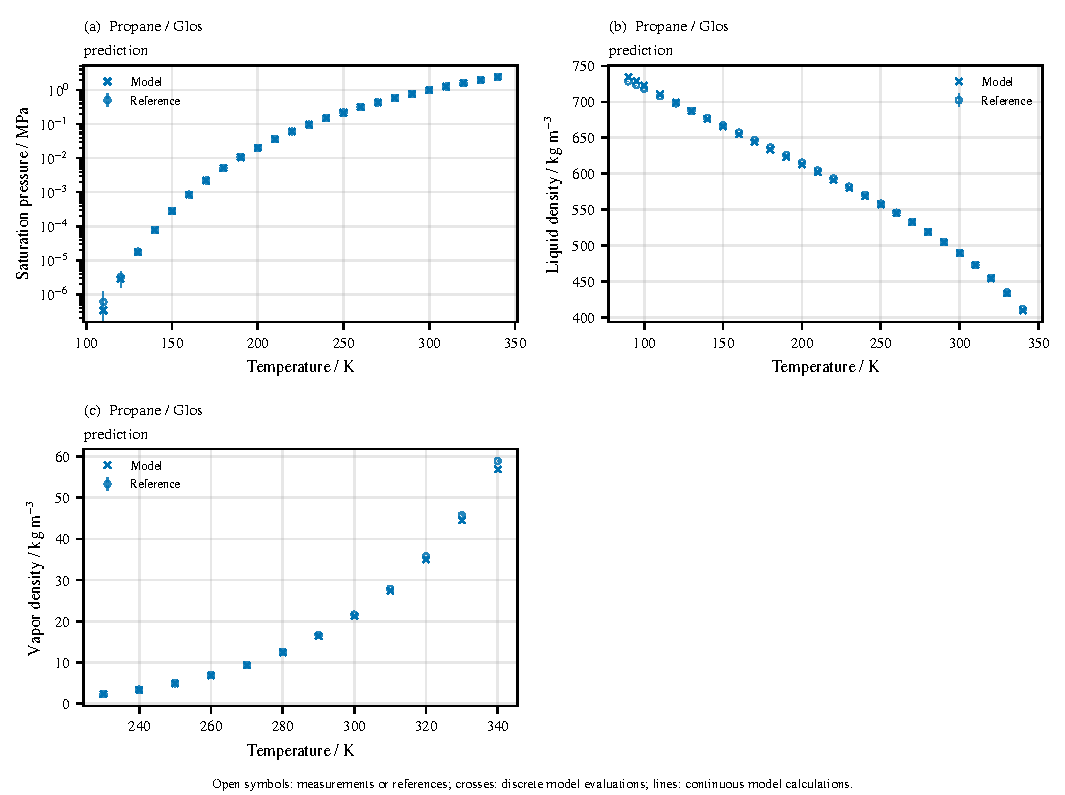
\includegraphics[page=1,width=\linewidth,height=19cm,keepaspectratio]{F8-pure-fluids}
\caption{Propane saturation pressure, saturated-liquid density and saturated-vapor density with the Gross--Sadowski parameters against the measurements of Glos et al., 90--340~K, with expanded measurement uncertainties (prediction)~\citep{Gross2001,Glos2004}.}
\label{fig:si-F8-pure-fluids-1}
\end{figure}
\clearpage

\begin{figure}[pos=p]
\centering
\includegraphics[page=2,width=\linewidth,height=19cm,keepaspectratio]{F8-pure-fluids}
\caption{Saturation pressures calculated for each of the 78 compounds of Gross and Sadowski; no measured reference is compared (numerical verification)~\citep{Gross2001}.}
\label{fig:si-F8-pure-fluids-2}
\end{figure}
\clearpage

\begin{figure}[pos=p]
\centering
\includegraphics[page=3,width=\linewidth,height=19cm,keepaspectratio]{F8-pure-fluids}
\caption{Saturated-liquid densities of diethyl ether, methane, propylene and toluene against measurements and digitized source-model values; diamonds mark the coldest states, where pressure closure failed~\citep{Gross2001}.}
\label{fig:si-F8-pure-fluids-3}
\end{figure}
\clearpage



\begin{figure}[pos=p]
\centering
\includegraphics[page=6,width=\linewidth,height=19cm,keepaspectratio]{F8-pure-fluids}
\caption{Saturation pressures of carbon dioxide, 220--300~K, and benzene, 290--540~K, with the quadrupolar parameters of Gross against the Span--Wagner reference equation and a DIPPR-101-form correlation; carbon dioxide also with nonpolar parameters (published-model reproduction)~\citep{grossEquationofstateContributionPolar2005,spanNewEquationState1996}.}
\label{fig:si-F8-pure-fluids-5}
\end{figure}
\clearpage

\begin{figure}[pos=p]
\centering
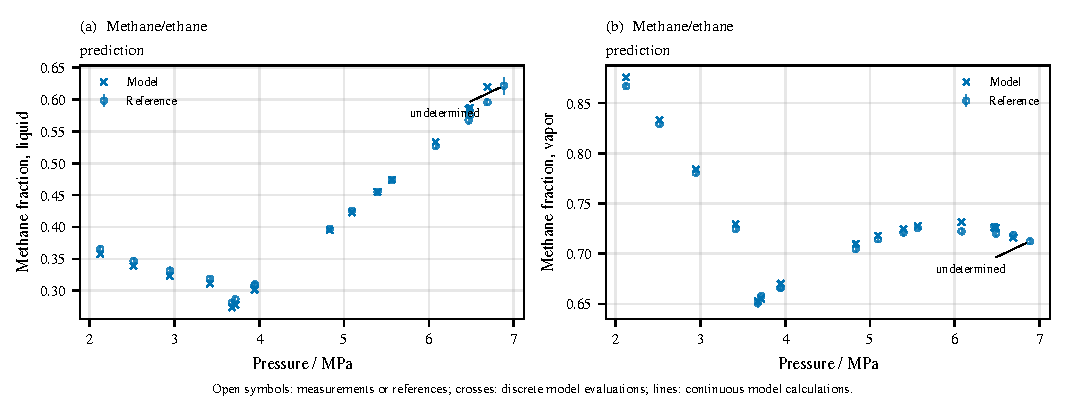
\includegraphics[page=1,width=\linewidth,height=19cm,keepaspectratio]{F9-neutral-mixtures}
\caption{Methane/ethane liquid and vapor methane fractions against the measurements of May et al., 203--244~K and 2.1--6.9~MPa, predicted with the Gross--Sadowski parameters and $k_{ij}=0$; one state is unavailable (prediction)~\citep{May2015,Gross2001}.}
\label{fig:si-F9-neutral-mixtures-1}
\end{figure}
\clearpage



\begin{figure}[pos=p]
\centering
\includegraphics[page=3,width=\linewidth,height=19cm,keepaspectratio]{F9-neutral-mixtures}
\caption{Liquid carbon dioxide fraction of carbon dioxide/THF at 313.2--353.2~K against the measurements and published model values of Schick et al.~\citep{Schick2023}.}
\label{fig:si-F9-neutral-mixtures-3}
\end{figure}
\clearpage

\begin{figure}[pos=p]
\centering
\includegraphics[page=4,width=\linewidth,height=19cm,keepaspectratio]{F9-neutral-mixtures}
\caption{Gross--Sadowski binary systems with the source's binary interactions: methane/butane, ethane/decane, ethane/diethyl ether, propane/benzene, carbon dioxide/decane, carbon dioxide/cyclohexane and hexane/1-chlorobutane, against measurements and digitized source-model values~\citep{Gross2001}.}
\label{fig:si-F9-neutral-mixtures-4}
\end{figure}
\clearpage

\begin{figure}[pos=p]
\centering
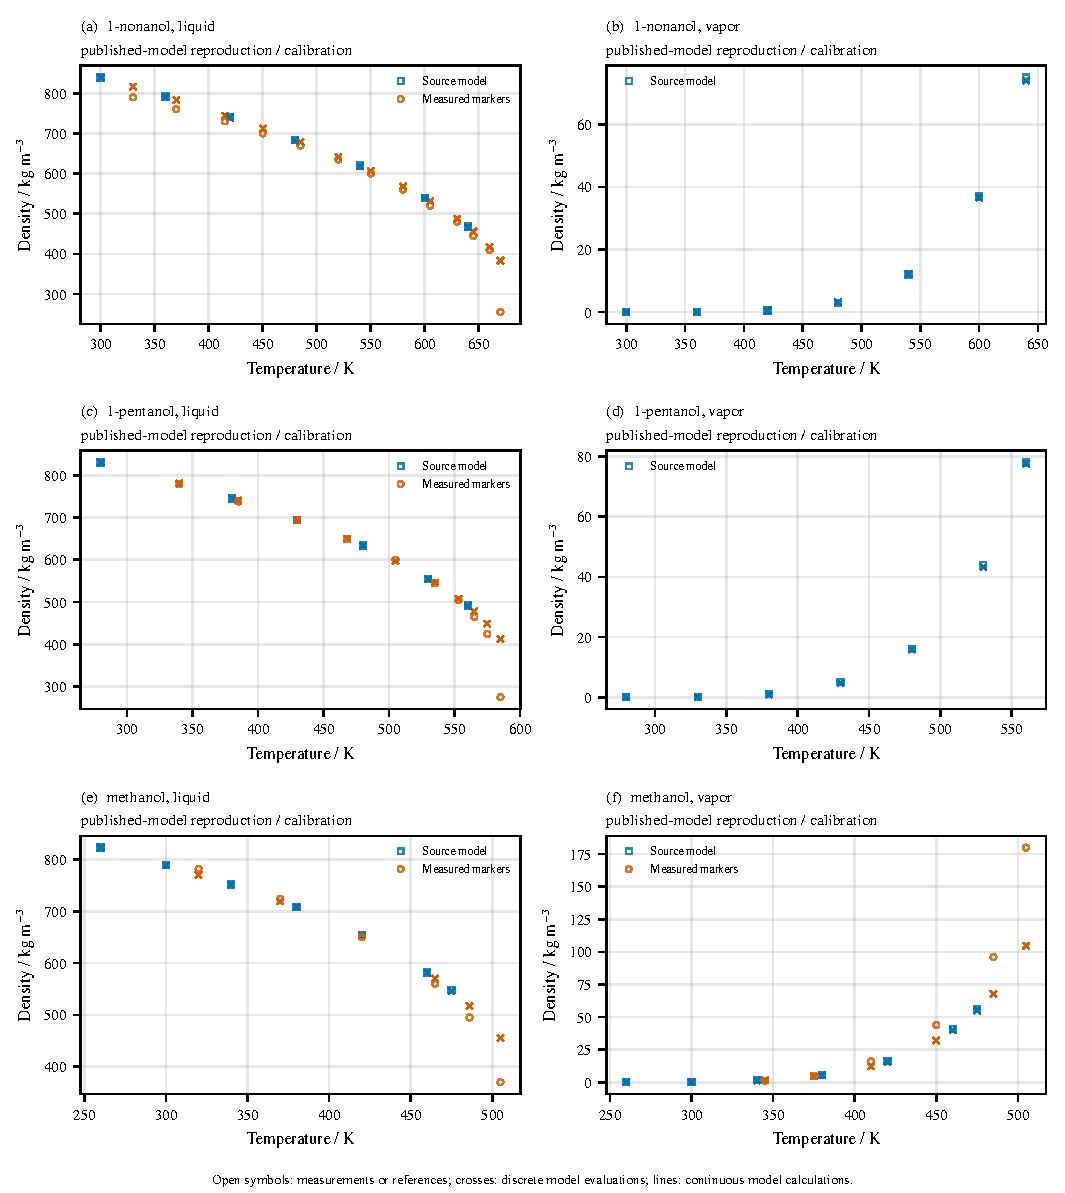
\includegraphics[page=1,width=\linewidth,height=19cm,keepaspectratio]{F10-associating}
\caption{Saturated-liquid and saturated-vapor densities of 1-nonanol, 1-pentanol and methanol with the Gross--Sadowski associating parameters, against measurements and digitized source-model values~\citep{Gross2002}.}
\label{fig:si-F10-associating-1}
\end{figure}
\clearpage

\begin{figure}[pos=p]
\centering
\includegraphics[page=2,width=\linewidth,height=19cm,keepaspectratio]{F10-associating}
\caption{Associating binary systems with the Gross--Sadowski parameters: isobutane/methanol, 1-propanol/ethylbenzene, 1-pentanol/benzene, 1-propanol/benzene, 2-propanol/benzene, butane/1-butanol, butane/ethanol, methanol/cyclohexane and methanol/1-octanol~\citep{Gross2002}.}
\label{fig:si-F10-associating-2}
\end{figure}
\clearpage





\begin{figure}[pos=p]
\centering
\includegraphics[page=2,width=\linewidth,height=19cm,keepaspectratio]{F11-aqueous-electrolytes}
\caption{Held et al.\ aqueous salt series, page 1 of five: solution density differences, vapor pressures, water activities and mean ionic activity coefficients of the 19 salts at 293.15--333.15~K, each against measurements and the digitized source-model curve; bars are the reading intervals of digitized values~\citep{Held2008}.}
\label{fig:si-F11-aqueous-electrolytes-2}
\end{figure}
\clearpage

\begin{figure}[pos=p]
\centering
\includegraphics[page=3,width=\linewidth,height=19cm,keepaspectratio]{F11-aqueous-electrolytes}
\caption{Held et al.\ aqueous salt series, page 2 of five: solution density differences, vapor pressures, water activities and mean ionic activity coefficients of the 19 salts at 293.15--333.15~K, each against measurements and the digitized source-model curve; bars are the reading intervals of digitized values~\citep{Held2008}.}
\label{fig:si-F11-aqueous-electrolytes-3}
\end{figure}
\clearpage

\begin{figure}[pos=p]
\centering
\includegraphics[page=4,width=\linewidth,height=19cm,keepaspectratio]{F11-aqueous-electrolytes}
\caption{Held et al.\ aqueous salt series, page 3 of five: solution density differences, vapor pressures, water activities and mean ionic activity coefficients of the 19 salts at 293.15--333.15~K, each against measurements and the digitized source-model curve; bars are the reading intervals of digitized values~\citep{Held2008}.}
\label{fig:si-F11-aqueous-electrolytes-4}
\end{figure}
\clearpage

\begin{figure}[pos=p]
\centering
\includegraphics[page=5,width=\linewidth,height=19cm,keepaspectratio]{F11-aqueous-electrolytes}
\caption{Held et al.\ aqueous salt series, page 4 of five: solution density differences, vapor pressures, water activities and mean ionic activity coefficients of the 19 salts at 293.15--333.15~K, each against measurements and the digitized source-model curve; bars are the reading intervals of digitized values~\citep{Held2008}.}
\label{fig:si-F11-aqueous-electrolytes-5}
\end{figure}
\clearpage

\begin{figure}[pos=p]
\centering
\includegraphics[page=6,width=\linewidth,height=19cm,keepaspectratio]{F11-aqueous-electrolytes}
\caption{Held et al.\ aqueous salt series, page 5 of five: solution density differences, vapor pressures, water activities and mean ionic activity coefficients of the 19 salts at 293.15--333.15~K, each against measurements and the digitized source-model curve; bars are the reading intervals of digitized values~\citep{Held2008}.}
\label{fig:si-F11-aqueous-electrolytes-6}
\end{figure}
\clearpage

\begin{figure}[pos=p]
\centering
\includegraphics[page=7,width=\linewidth,height=19cm,keepaspectratio]{F11-aqueous-electrolytes}
\caption{Practical osmotic coefficients with the Held 2014 parameters: NaCl, KCl and KBr at 298.15~K under both parameter strategies, and NaCl and KCl at 273.15~K, against the source-model curves and measurements~\citep{Held2014}.}
\label{fig:si-F11-aqueous-electrolytes-7}
\end{figure}
\clearpage

\begin{figure}[pos=p]
\centering
\includegraphics[page=8,width=\linewidth,height=19cm,keepaspectratio]{F11-aqueous-electrolytes}
\caption{Aqueous NaCl at 298.15~K: mean ionic activity coefficients fitted at or below 2~mol/kg and predicted above it, and relative permittivity. F0, published Figiel parameters with ion suppression; F1, D1 and P1, refits with the ion-suppression, density--temperature and dipolar-perturbation relations~\citep{Figiel2025,Yang2024,Rueben2024}.}
\label{fig:si-F11-aqueous-electrolytes-8}
\end{figure}
\clearpage











\begin{figure}[pos=p]
\centering
\includegraphics[page=2,width=\linewidth,height=19cm,keepaspectratio]{F4-phase-envelope}
\caption{Discrete comparisons of methane/ethane critical points and bubble and dew points with FeOs and teqp at their own compositions (numerical verification).}
\label{fig:si-F4-phase-envelope-2}
\end{figure}
\clearpage

\begin{figure}[pos=p]
\centering
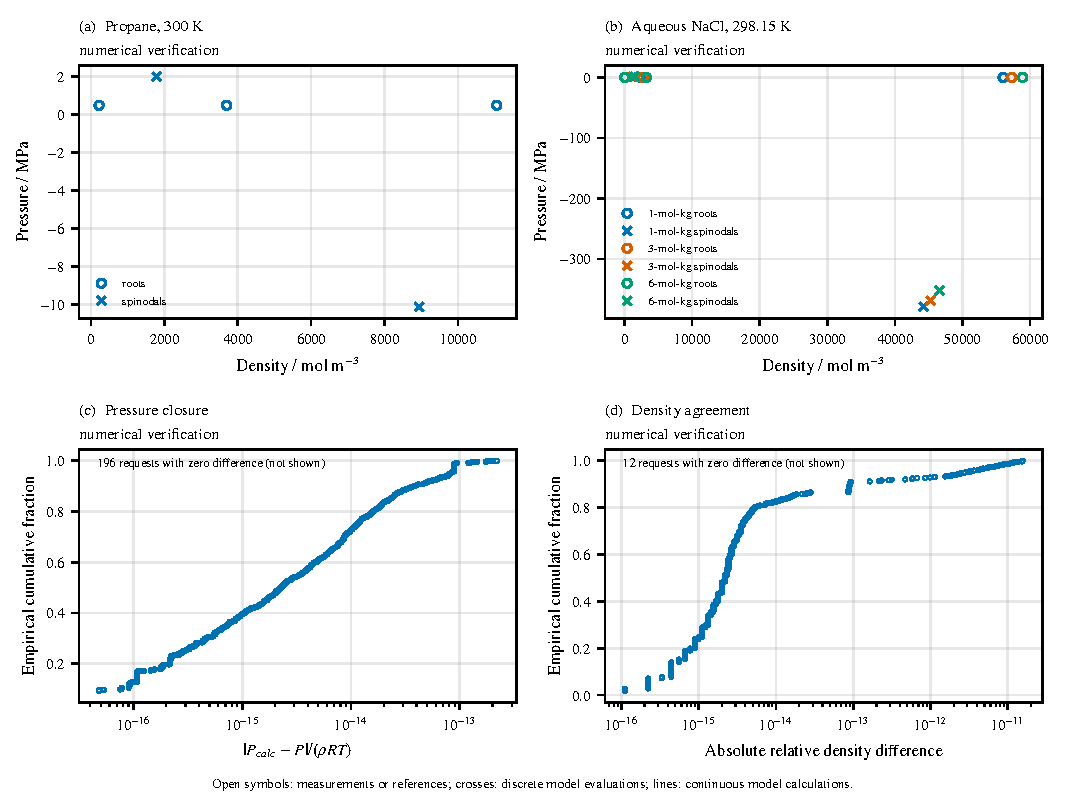
\includegraphics[page=1,width=\linewidth,height=19cm,keepaspectratio]{F2-density-roots}
\caption{Density roots and pressure closure (numerical verification). Top: roots and spinodals found for propane at 300~K and 0.499~MPa and for aqueous NaCl at 298.15~K and 0.1~MPa at 1, 3 and 6~mol/kg. Bottom: cumulative distributions of the reduced pressure residual and of the relative density difference from the frozen reference over the benchmark requests; requests with zero difference cannot be drawn on the logarithmic axis and are counted on each panel.}
\label{fig:si-F2-density-roots-1}
\end{figure}
\clearpage
